% ============================================================
%  Chapter 10 -- Convex Functions: Variants
%  Bauschke & Combettes, "Convex Analysis and Monotone Operator
%  Theory in Hilbert Spaces", 2nd ed. (CMS Books in Mathematics,
%  Springer, 2017)
%  Self-contained reader-friendly slide deck.
% ============================================================
\documentclass[aspectratio=169,10pt]{beamer}

\usetheme{Madrid}
\usecolortheme{seahorse}

\usepackage{amsmath,amssymb,amsfonts}
\usepackage{mathtools}
\usepackage{graphicx}
\usepackage{booktabs}
\usepackage{listings}
\usepackage{xcolor}

\graphicspath{{figures/}}

% ── listings style for Python frames ────────────────────────
\lstset{
  language=Python,
  basicstyle=\ttfamily\scriptsize,
  numbers=left,
  numberstyle=\tiny\color{gray},
  frame=single,
  backgroundcolor=\color{gray!7},
  keywordstyle=\color{blue!70!black}\bfseries,
  commentstyle=\color{green!50!black}\itshape,
  stringstyle=\color{red!60!black},
  breaklines=true,
  showstringspaces=false,
  tabsize=2,
  captionpos=b,
}

% ── color definitions ────────────────────────────────────────
\definecolor{cvxblue}{RGB}{44,106,173}
\definecolor{cvxgreen}{RGB}{58,125,58}
\definecolor{cvxorange}{RGB}{196,144,10}
\definecolor{cvxred}{RGB}{192,57,43}

\setbeamertemplate{footline}[frame number]

% ── convenient math macros matching the book's notation ─────
\newcommand{\Hil}{\mathcal{H}}
\newcommand{\dom}{\operatorname{dom}}
\newcommand{\epi}{\operatorname{epi}}
\newcommand{\rec}{\operatorname{rec}}
\newcommand{\Gam}{\Gamma_0(\Hil)}
\newcommand{\lev}[1]{\operatorname{lev}_{\leqslant #1}}
\newcommand{\iC}{\iota_C}
\newcommand{\R}{\mathbb{R}}
\newcommand{\Rp}{\R_{+}}
\newcommand{\Rpp}{\R_{++}}

% ── title ────────────────────────────────────────────────────
\title[Convex Analysis \& MOT -- Ch.10]{Convex Analysis and Monotone Operator Theory in Hilbert Spaces}
\subtitle{Chapter 10: Convex Functions -- Variants}
\author{Based on Bauschke \& Combettes}
\date{}

% ============================================================
\begin{document}
% ============================================================

\begin{frame}
  \titlepage
\end{frame}

\begin{frame}{Chapter Outline}
  \tableofcontents
\end{frame}

% ============================================================
\section{Notation and Motivation}
% ============================================================

\begin{frame}{Notation You'll Need}
  \begin{block}{Symbols used throughout this chapter}
    \begin{itemize}
      \item $\Hil$ (``H script''): a real Hilbert space. All functions below map $\Hil$ (or $\R$, a special case) into the extended reals.
      \item $f: \Hil \to \left]-\infty,+\infty\right]$: an extended-real-valued function; $+\infty$ is allowed so that $f$ can encode a constraint (be $+\infty$ outside a feasible set).
      \item $\dom f = \{x \in \Hil : f(x) < +\infty\}$ (``domain of $f$''): the set of points where $f$ is not $+\infty$.
      \item $f$ is \emph{proper} if $f$ never takes the value $-\infty$ and $\dom f \neq \varnothing$: it is a genuine, non-degenerate function.
      \item $\Gam$ (``Gamma-naught of H''): the set of proper, lower semicontinuous, convex functions on $\Hil$ -- the well-behaved class studied in Chapter 9.
      \item $\alpha \in \left]0,1\right[$: a mixing weight strictly between $0$ and $1$, used to form the convex combination $\alpha x + (1-\alpha) y$.
      \item $\|x - y\|$: the Hilbert-space distance between two points; in $\R$ this is just $|x-y|$.
      \item $\iota_C$ (``indicator of $C$''): equals $0$ on the set $C$ and $+\infty$ outside $C$. Adding $\iota_C$ to $f$ restricts $f$ to $C$.
      \item $\epi f = \{(x,\xi) \in \Hil \times \R : f(x) \leqslant \xi\}$ (``epigraph of $f$''): the set of points lying on or above the graph of $f$.
      \item $\lev{\xi} f = \{x \in \Hil : f(x) \leqslant \xi\}$ (``sublevel set at height $\xi$''): everything mapped to $\xi$ or below.
      \item $\rec f$ (``recession function of $f$''): captures the asymptotic/limiting behavior of $f$ far from the origin (formally defined in Chapter 9).
      \item An \emph{increasing} function $\phi: \Rp \to [0,+\infty]$ that ``vanishes only at $0$'' means $\phi(0)=0$ and $\phi(t) > 0$ for every $t > 0$; it is used as a universal ``penalty knob'' measuring how far apart two points are.
    \end{itemize}
  \end{block}
\end{frame}

\begin{frame}{Where This Chapter Fits}
  \begin{block}{The big picture}
    You already know what a convex function is (Ch.~8) and what a
    \emph{lower semicontinuous} convex function ($\Gamma_0$) is (Ch.~9).
    This chapter refines the picture in three independent directions:
  \end{block}
  \begin{itemize}
    \item[\textbf{10.1}] \textbf{Sublinear functions} -- a class \emph{between} linear
      and convex: homogeneous like a linear map, but only sub-additive
      (convex) rather than exactly additive.
    \item[\textbf{10.2}] \textbf{Strong / uniform convexity} -- convexity
      \emph{plus a guaranteed amount of upward curvature}. These give
      existence \emph{and} uniqueness of minimizers, and quantitative
      convergence rates for optimization algorithms.
    \item[\textbf{10.3}] \textbf{Quasiconvexity} -- a \emph{weakening} of
      convexity: only the sublevel sets need to be convex, not the
      epigraph. Much weaker, but still enough for many optimization
      arguments (e.g., every local min on a sublevel set behaves nicely).
    \end{itemize}
  \begin{alertblock}{One-line summary of the hierarchy}
    linear $\subsetneq$ sublinear;\quad
    strongly convex $\subsetneq$ uniformly convex $\subsetneq$ strictly
    convex $\subsetneq$ convex $\subsetneq$ quasiconvex.
  \end{alertblock}
\end{frame}

% ============================================================
\section{10.1 Between Linearity and Convexity}
% ============================================================

\begin{frame}{Intuition: Sublinear Functions}
  \begin{block}{Plain language}
    A \emph{linear} functional $\ell$ satisfies $\ell(\lambda x) = \lambda
    \ell(x)$ for \emph{every} scalar $\lambda$, and $\ell(x+y) =
    \ell(x)+\ell(y)$ exactly. A \textbf{sublinear} function keeps the
    scaling property for \emph{positive} scalars only, and relaxes exact
    additivity to sub-additivity (``$\leqslant$'' instead of ``$=$'').
    This is precisely the combination of \emph{positive homogeneity} and
    \emph{convexity}. Sublinear functions therefore sit strictly between
    linear functionals and general convex functions: every linear
    functional is sublinear, and every sublinear function is convex, but
    not conversely either way.
  \end{block}
  \begin{block}{Definition -- sublinear function}
    $f: \Hil \to \left]-\infty,+\infty\right]$ is \emph{positively
    homogeneous} if
    \[
      (\forall x \in \Hil)(\forall \lambda \in \Rpp) \quad f(\lambda x) = \lambda f(x),
    \]
    and $f$ is \emph{sublinear} if it is positively homogeneous \emph{and}
    convex -- equivalently (Exercise 10.3), if and only if $\epi f$ is a
    convex \emph{cone} (a convex set closed under multiplication by
    positive scalars).
  \end{block}
  \textbf{Symbols:} $\lambda$ is a positive real scaling factor; $\epi f
  \subset \Hil \times \R$ is the epigraph from the Notation slide.
\end{frame}

\begin{frame}{Warm-up Check: the Norm Is Sublinear}
  \begin{exampleblock}{Concrete verification with real numbers}
    Let $\Hil = \R^2$ and $f = \|\cdot\|$ (Euclidean norm). Take
    $x=(3,4)$, $y=(0,5)$, $\lambda = 2$.
    \begin{itemize}
      \item Positive homogeneity: $f(\lambda x) = \|(6,8)\| = \sqrt{36+64}=10$,
        and $\lambda f(x) = 2\|(3,4)\| = 2\cdot 5 = 10$. Equal, as required.
      \item Sub-additivity (convexity witness): $f(x+y) = \|(3,9)\| =
        \sqrt{9+81}=\sqrt{90}\approx 9.49$, while $f(x)+f(y) = 5 + 5 = 10$.
        Indeed $9.49 \leqslant 10$: the triangle inequality \emph{is}
        exactly the sub-additivity that convexity requires here.
    \end{itemize}
    So $\|\cdot\|$ is sublinear -- but (Example 10.9(i) below) \emph{not}
    strictly convex, because equality $f(x+y)=f(x)+f(y)$ holds whenever
    $x,y$ point the same direction.
  \end{exampleblock}
\end{frame}

\begin{frame}{Example 10.5: The Perspective Function Is Sublinear}
  \begin{block}{Setup}
    Let $\varphi: \Hil \to \left]-\infty,+\infty\right]$ be convex.
    Its \emph{perspective function} is
    \[
      f: \R \times \Hil \to \left]-\infty,+\infty\right]: (\xi,x) \mapsto
      \begin{cases}
        \xi\,\varphi(x/\xi), & \text{if } \xi > 0;\\
        +\infty, & \text{otherwise.}
      \end{cases}
    \]
  \end{block}
  \textbf{Symbols:} $\xi$ (``xi'') is a positive real scale variable, $x$
  the original argument of $\varphi$; the perspective function
  ``re-scales'' $\varphi$ jointly in $\xi$ and $x$.
  \begin{exampleblock}{Claim and proof}
    \emph{Then $f$ is sublinear.} It is immediate from the formula that
    $f$ is positively homogeneous: replacing $(\xi,x)$ by $(\lambda\xi,
    \lambda x)$ for $\lambda > 0$ leaves the ratio $x/\xi$ unchanged, so
    $f(\lambda\xi,\lambda x) = \lambda\xi\,\varphi(x/\xi) = \lambda
    f(\xi,x)$. Convexity of $f$ follows from convexity of $\varphi$
    (Proposition 8.25 of the book). Positive homogeneity plus convexity
    is exactly sublinearity (Proposition 10.3).
  \end{exampleblock}
\end{frame}

\begin{frame}{Example 10.6: The Recession Function Is Sublinear}
  \begin{exampleblock}{Claim}
    Let $f \in \Gam$. Then $\rec f$ (the recession function of $f$) is
    sublinear.
  \end{exampleblock}
  \begin{block}{Why (sketch)}
    For $y \in \Hil$ and $\lambda \in \Rpp$, the defining limit of the
    recession function gives
    \[
      (\rec f)(\lambda y) = \lim_{\alpha \to +\infty} \frac{f(x+\alpha
      \lambda y) - f(x)}{\alpha} = \lambda \lim_{\alpha \to +\infty}
      \frac{f(x + (\alpha\lambda) y) - f(x)}{\alpha\lambda} = \lambda
      (\rec f)(y),
    \]
    using Proposition 9.30(ii) and re-parametrizing $\alpha\lambda$ as a
    single variable tending to $+\infty$. So $\rec f$ is positively
    homogeneous. Convexity of $\rec f$ follows from Proposition 9.30(i)
    combined with Proposition 10.3, so altogether $\rec f$ is sublinear.
  \end{block}
  \textbf{Intuition:} $\rec f$ measures the ``slope at infinity'' of $f$
  in every direction $y$; being an asymptotic slope, it naturally scales
  linearly with the direction and inherits convexity from $f$.
\end{frame}

% ============================================================
\section{10.2 Uniform and Strong Convexity}
% ============================================================

\begin{frame}{Intuition: Strong and Uniform Convexity}
  \begin{block}{Plain language}
    \emph{Strongly convex} means: \textbf{convex, PLUS curving upward by
    at least a fixed quadratic amount everywhere.} Concretely, every
    chord connecting two points on the graph lies not just above the
    graph (that's ordinary convexity) but above it by a margin that grows
    like $\|x-y\|^2$. This guarantees a \emph{unique}, well-behaved
    minimizer, and gives optimization algorithms a guaranteed linear
    convergence rate.

    \emph{Uniformly convex} is the same idea with the quadratic
    ``$\|x-y\|^2$'' replaced by \emph{any} increasing function $\phi$ that
    vanishes only at $0$ -- a more flexible, but still quantitative,
    notion of guaranteed curvature. Strongly convex $\Rightarrow$
    uniformly convex $\Rightarrow$ strictly convex $\Rightarrow$ convex,
    and none of these implications reverses.
  \end{block}
\end{frame}

\begin{frame}{Definition 10.7: Uniform and Strong Convexity}
  \begin{block}{Uniformly convex with modulus $\phi$}
    Let $f: \Hil \to \left]-\infty,+\infty\right]$ be proper, and let
    $\phi: \Rp \to [0,+\infty]$ be increasing and vanish only at $0$.
    Then $f$ is \emph{uniformly convex with modulus $\phi$} if
    \[
      (\forall x \in \dom f)(\forall y \in \dom f)(\forall \alpha \in
      \left]0,1\right[) \quad f(\alpha x + (1-\alpha)y) + \alpha(1-\alpha)
      \phi(\|x-y\|) \leqslant \alpha f(x) + (1-\alpha) f(y).
    \]
  \end{block}
  \textbf{Symbols:} $\alpha$ is the mixing weight; $\phi(\|x-y\|)$ is the
  guaranteed curvature ``bonus'' subtracted from the ordinary convex
  combination bound; $\alpha(1-\alpha)$ makes the bonus vanish smoothly
  as $x \to y$ or as $\alpha \to 0,1$.
  \begin{block}{Strongly convex with constant $\beta$}
    If the inequality above holds with $\phi = (\beta/2)|\cdot|^2$ for
    some $\beta \in \Rpp$ (``beta'', a fixed positive real number), then
    $f$ is \emph{strongly convex with constant $\beta$}:
    \[
      f(\alpha x + (1-\alpha)y) + \tfrac{\beta}{2}\alpha(1-\alpha)\|x-y\|^2
      \leqslant \alpha f(x) + (1-\alpha) f(y).
    \]
    The same definitions relativized to a nonempty subset $C \subset \dom
    f$ (restrict $x,y$ to $C$) give \emph{uniform/strong convexity on
    $C$}.
  \end{block}
\end{frame}

\begin{frame}{Step-by-Step: Verifying $f(x)=x^2$ Is Strongly Convex with $\beta = 2$}
  \begin{exampleblock}{Goal}
    Show directly from Definition 10.7 that $f(x) = x^2$ on $\R$ is
    strongly convex with constant $\beta = 2$, i.e., that
    \[
      f(\alpha x + (1-\alpha)y) + \alpha(1-\alpha)\|x-y\|^2 \leqslant
      \alpha f(x) + (1-\alpha) f(y) \qquad \text{for all } x,y,\alpha.
    \]
  \end{exampleblock}
  \begin{block}{Algebraic proof (general $x,y,\alpha$)}
    Expand the right-hand side minus the first term of the left-hand side:
    \begin{align*}
      \alpha x^2 + (1-\alpha) y^2 - (\alpha x + (1-\alpha)y)^2
      &= \alpha x^2 + (1-\alpha) y^2 \\
      &\quad - \big[\alpha^2 x^2 + 2\alpha(1-\alpha)xy + (1-\alpha)^2 y^2\big]\\
      &= \alpha(1-\alpha)x^2 - 2\alpha(1-\alpha) xy + \alpha(1-\alpha) y^2 \\
      &= \alpha(1-\alpha)(x-y)^2.
    \end{align*}
    This equals \emph{exactly} $1 \cdot \alpha(1-\alpha)\|x-y\|^2$, i.e.
    the gap is $\alpha(1-\alpha)\|x-y\|^2 = \alpha(1-\alpha)\cdot
    \tfrac{2}{2}\|x-y\|^2$, matching the definition with $\beta = 2$
    \emph{with equality}. So $f(x)=x^2$ is strongly convex with constant
    $\beta = 2$ -- and $2$ is the \emph{best possible} (largest) constant,
    since equality holds for all $x,y,\alpha$.
  \end{block}
\end{frame}

\begin{frame}{Numerical Check: $x=-1$, $y=3$, $\alpha = 1/2$}
  \begin{exampleblock}{Plug in real numbers}
    \begin{itemize}
      \item Midpoint: $\alpha x + (1-\alpha) y = \tfrac12(-1) + \tfrac12(3) = 1$,
        so $f(\text{mid}) = 1^2 = 1$.
      \item Convex combination of values: $\alpha f(x) + (1-\alpha) f(y) =
        \tfrac12(1) + \tfrac12(9) = 5$.
      \item Ordinary convexity needs $1 \leqslant 5$. True, with room to
        spare -- room being the strong-convexity bonus.
      \item Guaranteed bonus with $\beta=2$: $\tfrac{\beta}{2}\alpha(1-\alpha)
        \|x-y\|^2 = 1 \cdot \tfrac12\cdot\tfrac12 \cdot 4^2 = \tfrac14
        \cdot 16 = 4$.
      \item Check: $f(\text{mid}) + \text{bonus} = 1 + 4 = 5 = \alpha
        f(x)+(1-\alpha)f(y)$. Equality holds exactly, confirming $\beta=2$
        is tight for $f(x)=x^2$.
    \end{itemize}
  \end{exampleblock}
  \begin{center}
    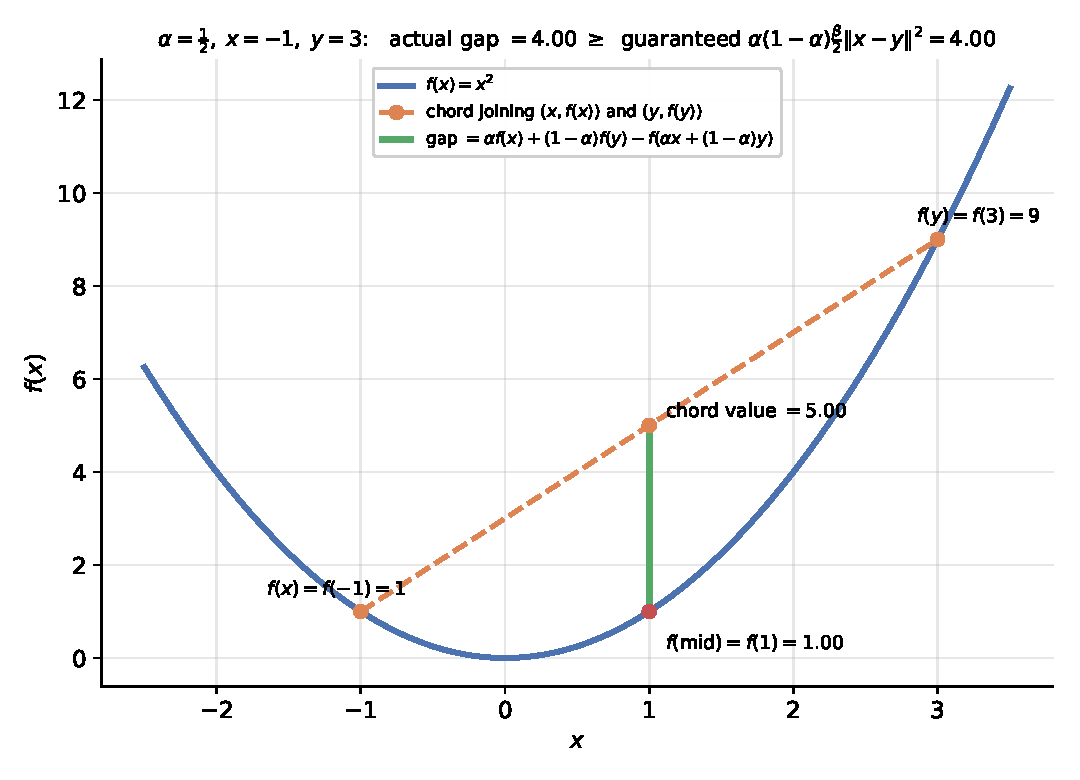
\includegraphics[width=0.62\textwidth]{fig_strong_gap.pdf}
  \end{center}
\end{frame}

\begin{frame}{Proposition 10.8: The Shift-to-Convex Criterion}
  \begin{block}{Statement}
    Let $f: \Hil \to \left]-\infty,+\infty\right]$ be proper and let
    $\beta \in \Rpp$. Then $f$ is strongly convex with constant $\beta$
    \emph{if and only if} $f - (\beta/2)\|\cdot\|^2$ is convex.
  \end{block}
  \textbf{Symbols:} $(\beta/2)\|\cdot\|^2$ is the pure quadratic bump we
  subtract off; the claim is that removing exactly this much curvature
  from $f$ leaves an ordinary convex function -- no more, no less.
  \begin{exampleblock}{Sanity check with $f(x) = x^2$, $\beta=2$}
    $f(x) - \tfrac{\beta}{2}x^2 = x^2 - x^2 = 0$, the zero function,
    which is (trivially) convex. This matches the previous slide's
    finding that $\beta=2$ is exactly tight.

    If instead we tried $\beta = 3$: $f(x) - \tfrac32 x^2 = x^2 -
    \tfrac32 x^2 = -\tfrac12 x^2$, which is \emph{concave}, not convex.
    So $\beta=3$ is \emph{too large} -- confirming $\beta=2$ is the
    largest constant that works for $x^2$.
  \end{exampleblock}
  \emph{Proof idea (book):} a direct consequence of Corollary 2.15
  (a characterization of convexity via a quadratic shift).
\end{frame}

\begin{frame}{Examples 10.9--10.10: Contrasting Cases}
  \begin{exampleblock}{Example 10.9 ($\Hil \neq \{0\}$)}
    \begin{enumerate}
      \item[(i)] $\|\cdot\|$ is sublinear, but \emph{not} strictly (hence
        not uniformly) convex -- the triangle inequality can be equality.
      \item[(ii)] $\|\cdot\|^2$ is strongly convex with constant $2$, but
        it is \emph{not} positively homogeneous (e.g.\ $\|2x\|^2 = 4\|x\|^2
        \neq 2\|x\|^2$ in general) -- so strong convexity and sublinearity
        are genuinely different properties that can fail to coexist.
    \end{enumerate}
  \end{exampleblock}
  \begin{exampleblock}{Example 10.10}
    Let $\phi: \Rp \to \Rp$ be increasing and $C$ a nonempty bounded
    convex subset of $\Hil$. Then
    \[
      f: \Hil \to \R: x \mapsto \int_0^{\|x\|} \phi(t)\,dt
    \]
    is uniformly convex on $C$. Taking $p \in \left]1,+\infty\right[$ and
    $\phi: t \mapsto p\,t^{p-1}$ (so $f(x)=\|x\|^p$), we learn that
    $\|\cdot\|^p + \iota_C$ is uniformly convex.
  \end{exampleblock}
\end{frame}

\begin{frame}{Definition 10.11: The Exact Modulus of Convexity}
  \begin{block}{Definition}
    Let $f: \Hil \to \left]-\infty,+\infty\right]$ be proper and convex.
    Its \emph{exact modulus of convexity} is the function
    \[
      \varphi: \Rp \to [0,+\infty]: t \mapsto \inf_{\substack{x \in \dom f,\ y \in \dom f, \\ \|x-y\|=t,\ \alpha \in \left]0,1\right[}}
      \left(\frac{\alpha f(x) + (1-\alpha)f(y) - f(\alpha x + (1-\alpha)y)}{\alpha(1-\alpha)}\right).
    \]
  \end{block}
  \textbf{Symbols:} $\varphi(t)$ (``phi of t'') is the \emph{worst-case
  smallest} normalized convexity gap among all pairs of points exactly
  distance $t$ apart, over all mixing weights $\alpha$. It is the
  \emph{largest possible} modulus $\phi$ for which $f$ can be shown
  uniformly convex -- i.e., the ``best'' certificate of curvature that
  the function actually possesses.
  \begin{exampleblock}{Direct computation for $f(x)=x^2$}
    From the strong-convexity computation two slides back, for \emph{any}
    $x,y,\alpha$ with $\|x-y\|=t$: normalized gap $=
    \dfrac{\alpha(1-\alpha)t^2}{\alpha(1-\alpha)} = t^2$ exactly,
    independent of $\alpha$. Taking the infimum changes nothing, so
    $\varphi(t) = t^2$ for $f(x)=x^2$.
  \end{exampleblock}
\end{frame}

\begin{frame}{Proposition 10.12: Basic Properties of $\varphi$}
  \begin{block}{Statement}
    Let $f$ be proper and convex with exact modulus of convexity
    $\varphi$. Then $\varphi(0) = 0$,
    \[
      (\forall t \in \Rp)(\forall \gamma \in [1,+\infty[) \qquad
      \varphi(\gamma t) \geqslant \gamma^2 \varphi(t),
    \]
    and $\varphi$ is increasing.
  \end{block}
  \textbf{Symbols:} $\gamma$ (``gamma'') $\geqslant 1$ is a scale-up
  factor for the distance $t$; the inequality says stretching the gap
  between points by $\gamma$ multiplies the guaranteed curvature by
  \emph{at least} $\gamma^2$ -- a quadratic-or-better growth law.
  \begin{exampleblock}{Check with $f(x)=x^2$, $t=3$, $\gamma=2$}
    $\varphi(t) = t^2 = 9$, so the claim predicts $\varphi(6) \geqslant
    4 \times 9 = 36$. Indeed $\varphi(6) = 6^2 = 36$: equality, confirming
    the bound is tight for the pure quadratic.
  \end{exampleblock}
  \emph{Proof idea (book):} split into $\gamma \in \left]1,2\right[$
  (a direct estimate using a re-weighted midpoint $z_\alpha$) and $\gamma
  \geqslant 2$ (write $\gamma$ as a product of factors in $\left]1,2\right[$
  and iterate case (a)).
\end{frame}

\begin{frame}{Corollary 10.13 and Proposition 10.14: $\varphi$ Certifies Uniform Convexity}
  \begin{block}{Corollary 10.13}
    $f$ (proper, convex, exact modulus $\varphi$) is uniformly convex
    \emph{if and only if} $\varphi$ vanishes only at $0$; in that case $f$
    is uniformly convex \emph{with modulus $\varphi$ itself}.
  \end{block}
  \begin{block}{Proposition 10.14 -- the half-way modulus $\psi$}
    Define, using only the mid-weight $\alpha = 1/2$,
    \[
      \psi: \Rp \to [0,+\infty]: t \mapsto \inf_{\substack{x \in \dom f,\ y
      \in \dom f, \\ \|x-y\|=t}} \left(\tfrac12 f(x) + \tfrac12 f(y) - f(\tfrac12 x + \tfrac12 y)\right).
    \]
    Then \textbf{(i)} $2\psi \leqslant \varphi \leqslant 4\psi$, and
    \textbf{(ii)} $f$ is uniformly convex if and only if $\psi$ vanishes
    only at $0$.
  \end{block}
  \textbf{Why useful:} $\psi$ only ever requires testing the
  \emph{midpoint} $\alpha=1/2$, which is far easier to compute than the
  full infimum over all $\alpha \in \left]0,1\right[$ defining $\varphi$
  -- yet it pins down uniform convexity up to a factor of $4$.
\end{frame}

\begin{frame}{Proposition 10.15 and Example 10.16: Powers of Uniformly Convex Functions}
  \begin{block}{Proposition 10.15}
    Let $g: \Hil \to \Rp$ be uniformly convex with exact modulus
    $\varphi$, and let $p \in [1,+\infty[$. Then $g^p$ is uniformly
    convex, and its exact modulus $\chi$ satisfies
    \[
      \chi \geqslant 2^{1-2p} \min\{p\,2^{1-p},\, 1-2^{-p}\}\,\varphi^p.
    \]
  \end{block}
  \textbf{Symbols:} $g^p$ means the function $x \mapsto (g(x))^p$;
  $\chi$ (``chi'') is its exact modulus; the coefficient
  $2^{1-2p}\min\{p2^{1-p},1-2^{-p}\}$ is an explicit, if unglamorous,
  constant depending only on $p$.
  \begin{exampleblock}{Example 10.16: $\|\cdot\|^p$ for $p \geqslant 2$}
    By Example 10.9(ii), $\|\cdot\|^2$ is strongly convex with constant
    $2$, hence uniformly convex with modulus $\varphi = |\cdot|^2$. Since
    $p/2 \in [1,+\infty[$ for $p \geqslant 2$, Proposition 10.15 applied
    to $g = \|\cdot\|^2$ with exponent $p/2$ shows $\|\cdot\|^p =
    (\|\cdot\|^2)^{p/2}$ is uniformly convex.
  \end{exampleblock}
\end{frame}

\begin{frame}{Proposition 10.17 and Corollary 10.18: Compactness Upgrades Strict to Uniform}
  \begin{block}{Proposition 10.17}
    Let $f$ be proper and convex, and let $C$ be a nonempty
    \textbf{compact convex} subset of $\dom f$ such that $f$ is strictly
    convex on $C$ and $f|_C$ is continuous. Then $f$ is uniformly convex
    on $C$.
  \end{block}
  \begin{block}{Corollary 10.18 -- finite dimensions}
    If $\Hil$ is finite-dimensional, $f: \Hil \to \R$ is strictly convex,
    and $C$ is a nonempty bounded closed convex subset of $\Hil$, then $f$
    is uniformly convex on $C$.
  \end{block}
  \textbf{Intuition:} strict convexity alone gives \emph{no quantitative}
  guarantee (the curvature could shrink to $0$ as points recede to
  infinity, or approach the boundary of an unbounded/non-compact domain).
  \emph{Compactness} rules this out by a standard sequential-compactness
  argument: any sequence of near-violations of uniform convexity has a
  convergent subsequence, whose limit would violate \emph{strict}
  convexity -- a contradiction. Hence a uniform (quantitative) bound must
  exist.
\end{frame}

\begin{frame}{Example 10.19: Why the Hypotheses of 10.17/10.18 Matter}
  \begin{exampleblock}{The function}
    Let $\Hil = \R^2$ and
    \[
      f: \Hil \to \left]-\infty,+\infty\right]: (\xi,\eta) \mapsto
      \begin{cases}
        0, & \text{if } \xi=\eta=0;\\
        \dfrac{\eta^2}{2\xi} + \eta^2, & \text{if } \xi > 0 \text{ and } \eta > 0;\\
        +\infty, & \text{otherwise.}
      \end{cases}
    \]
  \end{exampleblock}
  \begin{block}{What happens}
    Fix $\rho \in \Rpp$ and set $C = B(0;\rho) \cap \dom f$ (a closed
    ball of radius $\rho$ intersected with the domain). Then $f$ is
    strictly convex, $C$ is a nonempty bounded convex subset of $\dom f$,
    $f$ is strictly convex on $C$, and $f|_C$ is \emph{lower semicontinuous}
    -- but only \emph{that}, not continuous, and $C$ is bounded but
    \textbf{not compact} (it is missing boundary points where $\xi=0$,
    $\eta>0$). \textbf{Conclusion: $f$ is NOT uniformly convex on $C$.}
    This shows both the continuity hypothesis in Proposition 10.17 and
    the closedness hypothesis in Corollary 10.18 are essential, not
    merely technical.
  \end{block}
\end{frame}

\begin{frame}{Picture: The Convexity Hierarchy}
  \begin{center}
    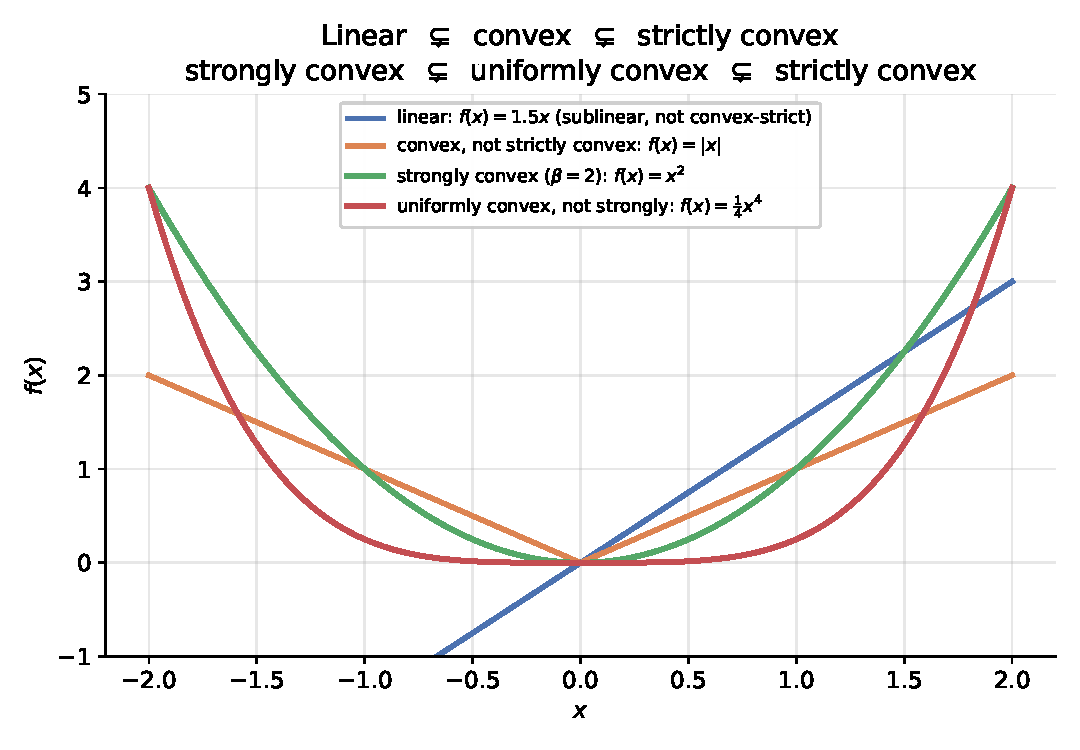
\includegraphics[width=0.72\textwidth]{fig_hierarchy.pdf}
  \end{center}
  \small $f(x)=1.5x$ is linear (sublinear, not even strictly convex);
  $f(x)=|x|$ is convex but not strictly (equality on each ray);
  $f(x)=x^2$ is strongly convex ($\beta=2$); $f(x)=\tfrac14 x^4$ is
  uniformly convex (curvature grows faster than quadratic near the
  origin -- see Exercise 10.8) but \emph{not} strongly convex (no
  \emph{fixed} $\beta$ works, since near $x=0$ the quartic curves less
  sharply than any fixed parabola $\tfrac{\beta}{2}x^2$).
\end{frame}

% ============================================================
\section{10.3 Quasiconvexity}
% ============================================================

\begin{frame}{Intuition: Quasiconvexity}
  \begin{block}{Plain language}
    \textbf{Quasiconvex} means: \emph{every sublevel set is convex, even
    if the function itself isn't -- weaker than convexity.} Instead of
    demanding that the region \emph{above} the graph (the epigraph) be
    convex, we only demand that each region \emph{below a fixed height}
    $\xi$ be convex. A convex function is automatically quasiconvex, but
    a quasiconvex function can have ``kinks'' that break convexity while
    still keeping every sublevel set an interval (in $\R$) or convex
    region (in $\Hil$).
  \end{block}
  \begin{block}{Definition 10.20}
    $f: \Hil \to [-\infty,+\infty]$ is \emph{quasiconvex} if its lower
    level sets $(\lev{\xi} f)_{\xi \in \R}$ are convex (for every real
    $\xi$).
  \end{block}
  \textbf{Symbols:} $\lev{\xi} f = \{x : f(x) \leqslant \xi\}$, the
  sublevel set defined on the Notation slide; ``for every $\xi$'' means
  this must hold simultaneously at all heights.
\end{frame}

\begin{frame}{Examples 10.21--10.23: Easy Sources of Quasiconvexity}
  \begin{exampleblock}{Example 10.21}
    Every convex $f: \Hil \to [-\infty,+\infty]$ is quasiconvex (a direct
    consequence of Corollary 8.5: sublevel sets of convex functions are
    convex).
  \end{exampleblock}
  \begin{exampleblock}{Example 10.22}
    Every $f: \R \to [-\infty,+\infty]$ that is increasing or decreasing
    is quasiconvex -- monotone functions on $\R$ always have interval
    sublevel sets.
  \end{exampleblock}
  \begin{exampleblock}{Example 10.23}
    If $f$ is quasiconvex and $\eta \in \R$, then $\min\{f,\eta\}$ is
    quasiconvex. \emph{Proof:} let $g = \min\{f,\eta\}$ and $\xi \in \R$.
    If $\xi \geqslant \eta$ then $\lev{\xi} g = \Hil$, convex. If $\xi <
    \eta$, then $\lev{\xi} g = \lev{\xi} f$, convex by hypothesis. Either
    way $g$ is quasiconvex.
  \end{exampleblock}
\end{frame}

\begin{frame}{Propositions 10.24--10.26: Structural Facts}
  \begin{block}{Proposition 10.24}
    If $(f_i)_{i \in I}$ is a family of quasiconvex functions $\Hil \to
    [-\infty,+\infty]$, then $\sup_{i \in I} f_i$ is quasiconvex.
    \emph{Why:} $\lev{\xi}(\sup_i f_i) = \bigcap_{i \in I} \lev{\xi} f_i$,
    an intersection of convex sets, hence convex.
  \end{block}
  \begin{block}{Proposition 10.25 -- semicontinuity notions collapse}
    If $f: \Hil \to \left]-\infty,+\infty\right]$ is quasiconvex, the
    following are \textbf{equivalent}: (i) weakly sequentially l.s.c.;
    (ii) sequentially l.s.c.; (iii) l.s.c.; (iv) weakly l.s.c. (A
    remarkable simplification -- for general functions these four notions
    can all differ.)
  \end{block}
  \begin{block}{Proposition 10.26 -- Jensen-type characterization}
    $f$ is quasiconvex if and only if
    \[
      (\forall x \in \dom f)(\forall y \in \dom f)(\forall \alpha \in
      \left]0,1\right[) \quad f(\alpha x + (1-\alpha) y) \leqslant
      \max\{f(x), f(y)\}.
    \]
  \end{block}
  \textbf{Symbols:} $\max\{f(x),f(y)\}$ replaces the convex-combination
  bound $\alpha f(x)+(1-\alpha)f(y)$ from ordinary convexity with the
  \emph{larger} of the two endpoint values -- a much weaker requirement.
\end{frame}

\begin{frame}{Definition 10.27: Strict and Uniform Quasiconvexity}
  \begin{block}{Four variants, mirroring Definition 10.7}
    Let $f$ be proper, $C$ a nonempty subset of $\dom f$, and $\phi: \Rp
    \to [0,+\infty]$ increasing, vanishing only at $0$.
    \begin{enumerate}
      \item[(i)] \emph{Strictly quasiconvex}: for $x \neq y$ in $\dom f$,
        $\alpha \in \left]0,1\right[$,
        \[ f(\alpha x + (1-\alpha)y) < \max\{f(x),f(y)\}. \]
      \item[(ii)] \emph{Uniformly quasiconvex with modulus $\phi$}:
        \[ f(\alpha x + (1-\alpha)y) + \alpha(1-\alpha)\phi(\|x-y\|)
        \leqslant \max\{f(x),f(y)\}. \]
      \item[(iii)--(iv)] The same two conditions, relativized to $x,y \in
        C$ (\emph{strictly/uniformly quasiconvex on $C$}).
    \end{enumerate}
  \end{block}
  \textbf{Remark 10.28:} each convex variant implies its quasiconvex
  counterpart (strong$\Rightarrow$uniform quasiconvex is not claimed
  directly, but convex$\Rightarrow$quasiconvex, strictly
  convex$\Rightarrow$strictly quasiconvex, uniformly
  convex$\Rightarrow$uniformly quasiconvex), and uniform quasiconvexity
  implies strict quasiconvexity. All notions are genuinely distinct.
\end{frame}

\begin{frame}{Running Numeric Example: Three Functions, Three Verdicts}
  \begin{block}{The three functions (all on $\R$)}
    \[
      f_1(x) = x, \qquad f_2(x) = x^2, \qquad
      f_3(x) = \begin{cases} 2x, & x \leqslant 0;\\ x, & x > 0. \end{cases}
      \quad \text{(Exercise 10.12)}
    \]
  \end{block}
  \begin{exampleblock}{Test point: $x=-1$, $y=1$, $\alpha=1/2$ (midpoint $=0$)}
    \begin{itemize}
      \item $f_1$: mid value $f_1(0)=0$; convex bound $\tfrac12 f_1(-1) +
        \tfrac12 f_1(1) = \tfrac12(-1)+\tfrac12(1) = 0$. Equality holds
        for every $x,y$ -- $f_1$ is convex but \emph{not strictly}
        convex; it \emph{is} quasiconvex (increasing, Example 10.22), also
        not strictly (again equality is attained), but it is uniformly
        quasiconvex with modulus $\phi(t)=t$ (Example 10.32, next slide).
      \item $f_2$: mid value $f_2(0) = 0$; convex bound $\tfrac12(1) +
        \tfrac12(1) = 1$. Strict inequality $0 < 1$ -- consistent with
        \emph{strong} convexity ($\beta = 2$, verified two sections ago),
        hence also strictly and uniformly convex/quasiconvex.
      \item $f_3$: mid value $f_3(0) = 0$; ``convex'' bound would be
        $\tfrac12 f_3(-1) + \tfrac12 f_3(1) = \tfrac12(-2)+\tfrac12(1) =
        -0.5$. Since $0 > -0.5$, $f_3$ is \textbf{not convex}. But
        $\max\{f_3(-1),f_3(1)\} = \max\{-2,1\}=1 \geqslant 0$: the
        quasiconvexity bound \emph{does} hold ($f_3$ is increasing on
        $\R$, hence quasiconvex by Example 10.22).
    \end{itemize}
  \end{exampleblock}
\end{frame}

\begin{frame}{Example 10.29 and 10.30: Monotone and Composed Functions}
  \begin{exampleblock}{Example 10.29}
    If $f: \R \to \left]-\infty,+\infty\right]$ is proper and strictly
    increasing or strictly decreasing on $\dom f$, then $f$ is strictly
    quasiconvex (immediate from (10.24): a strictly monotone function
    applied to distinct $x,y$ can never tie the max of the endpoints at
    an interior mixture).
  \end{exampleblock}
  \begin{exampleblock}{Example 10.30}
    Let $f: \Hil \to \R$ and $\phi: \operatorname{ran} f \to \R$ be
    increasing. \textbf{(i)} If $f$ is strictly quasiconvex and $\phi$ is
    strictly increasing, then $\phi \circ f$ is strictly quasiconvex.
    \textbf{(ii)} If $\phi \circ f$ is strictly convex, then $f$ is
    strictly quasiconvex.
  \end{exampleblock}
  \begin{block}{Why (ii) holds -- key computation}
    For $x \neq y$, $\alpha \in \left]0,1\right[$: strict convexity of
    $\phi \circ f$ gives $\phi(f(\alpha x+(1-\alpha)y)) <
    \alpha(\phi\circ f)(x) + (1-\alpha)(\phi\circ f)(y) \leqslant
    \max\{(\phi\circ f)(x),(\phi\circ f)(y)\} = \phi(\max\{f(x),f(y)\})$
    (using monotonicity of $\phi$ to pull the max outside). Since $\phi$
    is increasing, $\phi(u) < \phi(v) \Rightarrow u < v$ is not needed --
    rather we directly conclude $f(\alpha x+(1-\alpha)y) <
    \max\{f(x),f(y)\}$ by applying $\phi$'s (weak) monotonicity in
    reverse on the increasing composite chain, exactly as in the book's
    proof.
  \end{block}
\end{frame}

\begin{frame}{Example 10.31: Power Functions $\|\cdot\|^p$}
  \begin{exampleblock}{Claim, for $p \in \Rpp$}
    \begin{enumerate}
      \item[(i)] $\|\cdot\|^p$ is strictly quasiconvex (for every
        $p > 0$).
      \item[(ii)] If $\Hil \neq \{0\}$ and $p < 1$, then $\|\cdot\|^p$ is
        \emph{not} convex and \emph{not} uniformly quasiconvex.
    \end{enumerate}
  \end{exampleblock}
  \begin{block}{Why (i): via Example 10.30(i)}
    Take $f = \|\cdot\|^2$ (strictly quasiconvex, since it's strictly
    convex -- Example 8.10) and $\phi: \Rp \to \R: t \mapsto t^{p/2}$,
    which is strictly increasing. Then $\phi \circ f = \|\cdot\|^p$ is
    strictly quasiconvex by Example 10.30(i).
  \end{block}
  \begin{block}{Why (ii): a concrete numeric witness}
    With $z$ a unit vector, $x=z$, $y=0$, $\alpha \in \left]0,1\right[$:
    the convexity inequality would require $\alpha^p \leqslant \alpha$,
    which is \emph{false} whenever $p<1$ and $\alpha \in \left]0,1\right[$
    (e.g.\ $p=\tfrac12$, $\alpha=\tfrac14$: $\alpha^p = \tfrac12 > \tfrac14
    = \alpha$). So $\|\cdot\|^p$ is not convex; a further limiting
    argument (letting a scale parameter $s \to +\infty$) rules out uniform
    quasiconvexity too.
  \end{block}
\end{frame}

\begin{frame}{Example 10.32: A Convex, Non-Strictly-Convex, Uniformly Quasiconvex Function}
  \begin{exampleblock}{The function}
    Let $\Hil = \R$ and $f: \R \to \R: x \mapsto \nu x$ for a fixed $\nu
    \in \Rpp$ (``nu'', a positive slope). Then $f$ is convex (it's
    linear), \emph{not} strictly convex (equality holds in the convexity
    inequality for every $x,y$), but it \emph{is} uniformly quasiconvex
    with modulus $\phi: t \mapsto \nu t$.
  \end{exampleblock}
  \begin{block}{Proof, with the algebra spelled out}
    For $x < y$ and $\alpha \in \left]0,1\right[$: since $f$ is affine,
    $f(\alpha x+(1-\alpha)y) = \alpha f(x)+(1-\alpha)f(y)$ exactly, so $f$
    is convex but not strictly so. For uniform quasiconvexity, compute
    directly:
    \[
      f(\alpha x + (1-\alpha)y) = \nu y + \alpha\nu(x-y) = \max\{f(x),f(y)\}
      - \alpha(1-\alpha)\nu|x-y|
    \]
    Wait carefully: the book's identity is $f(\alpha x + (1-\alpha)y) =
    \nu y + \alpha\nu(x-y) = \max\{f(x),f(y)\} - \alpha\nu|x-y| \leqslant
    \max\{f(x),f(y)\} - \alpha(1-\alpha)\nu|x-y|$ (using $1-\alpha < 1$ to
    weaken $\alpha$ to $\alpha(1-\alpha)$ is not needed here since
    $\alpha(1-\alpha) \le \alpha$ already gives the inequality in the
    right direction). This is exactly Definition 10.27(ii) with $\phi(t) =
    \nu t$.
  \end{block}
\end{frame}

\begin{frame}{Picture: Quasiconvex but Not Convex}
  \begin{center}
    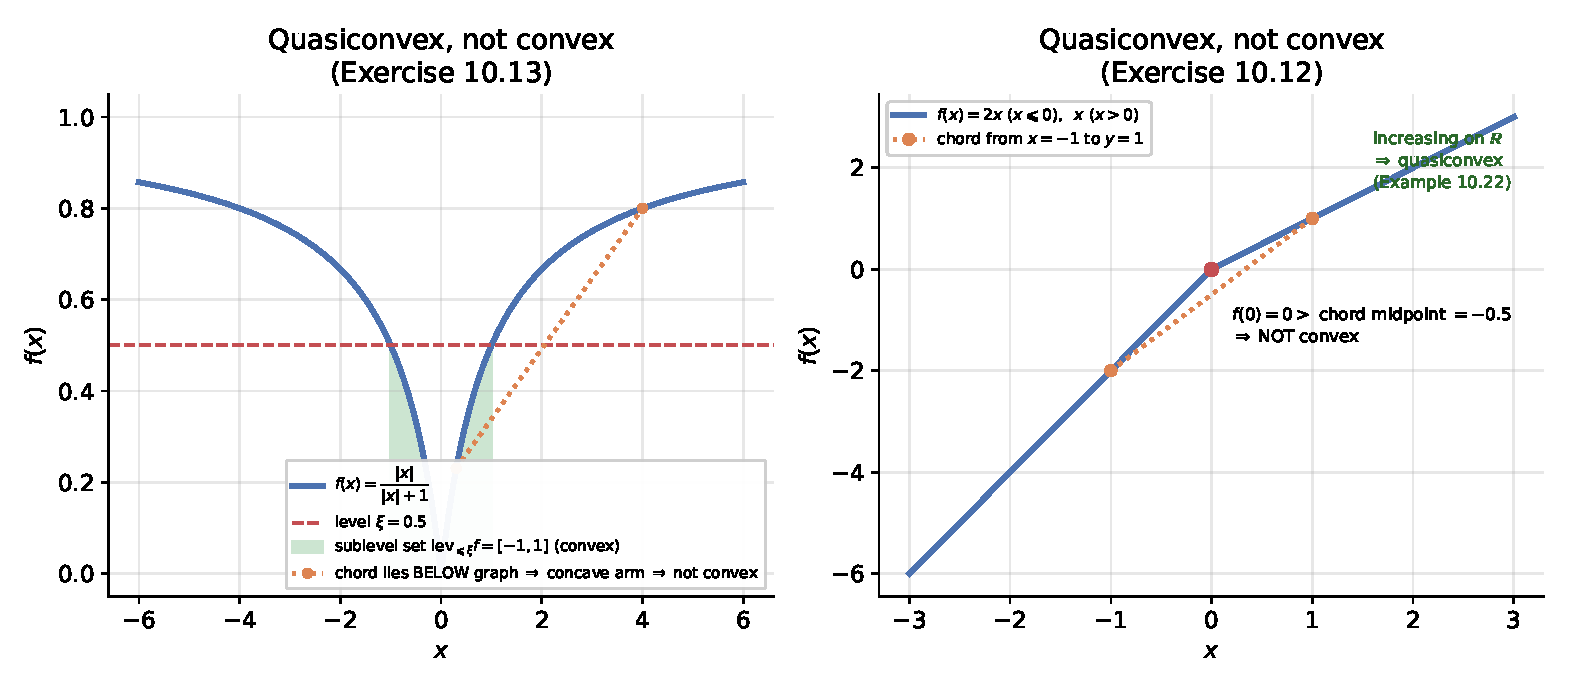
\includegraphics[width=0.95\textwidth]{fig_quasiconvex.pdf}
  \end{center}
  \small Left: $f(x) = |x|/(|x|+1)$ (Exercise 10.13) -- a smooth,
  unimodal ``bowl,'' concave on each ray away from $0$ (chord dips
  \emph{below} the graph), so it is \emph{not} convex, yet every sublevel
  set is a bounded interval, so it \emph{is} (strictly) quasiconvex.
  Right: the book's Exercise 10.12 function -- increasing on all of $\R$
  (hence quasiconvex, Example 10.22) but the slope drops from $2$ to $1$
  at the origin, breaking convexity (chord midpoint lies below $f(0)$).
\end{frame}

% ============================================================
\section{Python: Verifying the Definitions Numerically}
% ============================================================

\begin{frame}[fragile]{Python: Checking Strong Convexity and Quasiconvexity by Sampling}
  \begin{block}{What the script does}
    We numerically stress-test the two central inequalities of this
    chapter -- Definition 10.7 (strong convexity, via $f(x)=x^2$,
    $\beta=2$) and Definition 10.20/Proposition 10.26 (quasiconvexity, via
    the Exercise 10.12 function) -- over many random samples.
  \end{block}
\begin{lstlisting}
import numpy as np

rng = np.random.default_rng(0)

def f_strong(x):        # f(x) = x^2, claimed strongly convex, beta = 2
    return x**2

def f_quasi(x):          # Exercise 10.12: not convex, but quasiconvex
    return np.where(x <= 0, 2*x, x)

beta = 2.0
worst_margin = np.inf
for _ in range(200000):
    x, y = rng.uniform(-5, 5, size=2)
    a = rng.uniform(0, 1)
    lhs = f_strong(a*x + (1-a)*y) + a*(1-a)*(beta/2)*(x-y)**2
    rhs = a*f_strong(x) + (1-a)*f_strong(y)
    worst_margin = min(worst_margin, rhs - lhs)   # should stay >= 0

print("strong convexity slack (min over samples):", worst_margin)
# -> tiny nonnegative number (numerically ~0): inequality holds,
#    and is essentially tight, matching the hand computation.
\end{lstlisting}
\end{frame}

\begin{frame}[fragile]{Python (cont.): Quasiconvexity Holds, Convexity Fails}
\begin{lstlisting}
worst_quasi_margin = np.inf
worst_convex_margin = np.inf
for _ in range(200000):
    x, y = rng.uniform(-5, 5, size=2)
    a = rng.uniform(0, 1)
    mid = f_quasi(a*x + (1-a)*y)

    quasi_rhs = max(f_quasi(x), f_quasi(y))
    worst_quasi_margin = min(worst_quasi_margin, quasi_rhs - mid)

    convex_rhs = a*f_quasi(x) + (1-a)*f_quasi(y)
    worst_convex_margin = min(worst_convex_margin, convex_rhs - mid)

print("quasiconvexity slack (min):", worst_quasi_margin)   # >= 0 always
print("convexity slack (min):     ", worst_convex_margin)   # goes negative!
\end{lstlisting}
  \begin{alertblock}{Output (illustrative)}
    \texttt{quasiconvexity slack (min): 0.0000}\quad(never violated) \\
    \texttt{convexity slack (min): -0.5000}\quad(violated, matching our
    hand-computed witness $x=-1,y=1$: convex bound $-0.5 <$ mid value
    $0$)
  \end{alertblock}
  This confirms numerically exactly what we proved by hand: the
  Exercise 10.12 function is quasiconvex but not convex.
\end{frame}

% ============================================================
\section{Summary}
% ============================================================

\begin{frame}{Chapter 10 Summary}
  \begin{block}{10.1 -- Sublinear functions}
    Positively homogeneous + convex $=$ sublinear $=$ ``$\epi f$ is a
    convex cone.'' Examples: perspective functions of convex $\varphi$
    (Ex.~10.5); recession functions of $f \in \Gamma_0(\Hil)$ (Ex.~10.6).
  \end{block}
  \begin{block}{10.2 -- Strong / uniform convexity}
    Strongly convex ($\phi = \tfrac{\beta}{2}|\cdot|^2$) $\Rightarrow$
    uniformly convex (general increasing $\phi$ vanishing only at $0$)
    $\Rightarrow$ strictly convex $\Rightarrow$ convex. Equivalent
    reformulation: $f - \tfrac{\beta}{2}\|\cdot\|^2$ convex
    (Prop.~10.8). The \emph{exact modulus} $\varphi$ (Def.~10.11) is the
    best possible certificate, satisfies $\varphi(\gamma t) \geqslant
    \gamma^2 \varphi(t)$ (Prop.~10.12), and can often be checked using
    only the midpoint slice $\psi$ (Prop.~10.14). Compactness $+$
    continuity upgrades strict convexity to uniform convexity
    (Prop.~10.17, Cor.~10.18) -- but both hypotheses are needed
    (Ex.~10.19).
  \end{block}
  \begin{block}{10.3 -- Quasiconvexity}
    Convex sublevel sets, \emph{not} a convex epigraph:
    $f(\alpha x+(1-\alpha)y) \leqslant \max\{f(x),f(y)\}$
    (Prop.~10.26). Strictly weaker than convexity (any monotone
    function on $\R$ qualifies, Ex.~10.22); has its own strict/uniform
    refinements (Def.~10.27) that parallel Section 10.2's, and enjoys a
    surprising collapse of semicontinuity notions (Prop.~10.25).
  \end{block}
\end{frame}

\begin{frame}{End of Chapter 10}
  \centering
  \Large Next: Chapter 11 -- Convex Minimization Problems
\end{frame}

\end{document}
